\documentclass[../../main.tex]{subfiles}
\begin{document}
\section{Modelling a Suspension Bridge: A Brief History}
A common and easy to understand concept of bridges are that ``The longer the bridge, the more pilots are needed''. But the foundation of bridges are expensive. Suspension bridges are a great solution, being able to span larger distances between pilots than conventional bridges. Since the construction of the first early suspension bridges, there have been multiple collapses. The Tacoma Bridge Narrows collapse being one of the most well-known. This has sparked curiosity in various disciplines such as applied mathematics and engineering.\\

Since the cables suspending the roadbed can only exert a force in a single direction, an asymmetric non-linearity occurs. A suspension bridge also consists of various structural parts. Therefore, the modelling of a suspension bridge can be a complex and difficult undertaking.


\section{Modelling a suspension bridge: An Engineering Example}
Consider a basic model for a suspension bridge given in [Yos04]. The bridge is a symmetric four-span suspension bridge. The study looks at the bending and torsional rigidity of the towers, the sag of the main cable and applied static loads.
\\ 

The bridge is divided into four parts, two main spans in the centre and two edge spans on either side. This configuration results in three supporting towers. The rigidity of the centre tower is determined by two parameters, $K_{tb}$ for the bending rigidity and $K_{tt}$ for the torsional rigidity. The force that the cables exert on the towers, are modelled as elastic springs. The parameter $K_c$ describes the force that the springs act on the towers. This value $K_c$ can act in both directions parallel to the span and is dependent on the length of the span.\\

Realistically, it is not possible for the main cable to have enough tension to remain horizontal. The main cable obtains the shape of a parabola. Any elastic elongation is assumed to be negligible. The reason for this is not given.\\

The transverse (vertical) deflection of the girder or roadbed, is mainly dependent of the shape of the parabola of the main cable. Any distortion in the main cable is reflected in the transverse motion of the girder. The maximum deflection occurs in the middle of a span.
\\

The roadbed is chosen as a ``streamlined twin-box girder'' which is a three dimensional structure which is aerodynamically stable. This is to counteract the well known effect that wind can have on these multi-span suspension bridges. The article of [Xu97] presents a similar supporting structure and reduces the structure to an equivalent beam.\\

\section{Simplified Mathematical Model for a Suspended Beam}
Consider the model of a basic single span suspension bridge. This specific model consists of a main span which is suspended, connected to a conventional bridge on either side. This is illustrated in Figure 7.1. \textcolor{red}{(Maputo-Katembe bridge)}.


\text{red}{*********Skuif dalk na chapter 1 as motiveering and verduidelik al die verskillende dele (beam, plate, membrane, roadbed, pilots, ens...}
\begin{figure}[h!]
 \centering
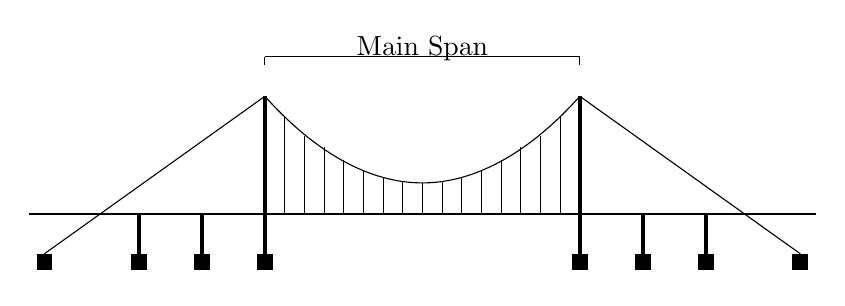
\begin{tikzpicture}
\draw (3,2) -- (7,2);
\draw (3,2) -- (3,1.9);
\draw (7,2) -- (7,1.9);
\node at (5,2.1) {Main Span};

\draw[line width = 0.25mm] (0,0) -- (10,0);

\draw[line width = 0.5mm] (1.4,0) -- (1.4,-0.5);
\draw[line width = 2mm] (1.4,-0.5) -- (1.4,-0.7);

\draw[line width = 0.5mm] (2.2,0) -- (2.2,-0.5);
\draw[line width = 2mm] (2.2,-0.5) -- (2.2,-0.7);

\draw[line width = 0.5mm] (8.6,0) -- (8.6,-0.5);
\draw[line width = 2mm] (8.6,-0.5) -- (8.6,-0.7);

\draw[line width = 0.5mm] (7.8,0) -- (7.8,-0.5);
\draw[line width = 2mm] (7.8,-0.5) -- (7.8,-0.7);

\draw[line width = 0.5mm] (3,1.5) -- (3,-0.5);
\draw[line width = 2mm] (3,-0.5) -- (3,-0.7);

\draw[line width = 0.5mm] (7,1.5) -- (7,-0.5);
\draw[line width = 2mm] (7,-0.5) -- (7,-0.7);

\draw (5,0.4) parabola (3,1.5);
\draw (5,0.4) parabola (7,1.5) ;

\draw (3,1.5) -- (0.2,-0.5);
\draw (7,1.5) -- (9.8,-0.5);

\draw[line width = 2mm] (0.2,-0.5) -- (0.2,-0.7);
\draw[line width = 2mm] (9.8,-0.5) -- (9.8,-0.7);


\draw[line width = 0.1mm] (5,0) -- (5,0.4);
\draw[line width = 0.1mm] (5.25,0) -- (5.25,0.43);
\draw[line width = 0.1mm] (5.5,0) -- (5.5,0.46);
\draw[line width = 0.1mm] (5.75,0) -- (5.75,0.55);
\draw[line width = 0.1mm] (6,0) -- (6,0.69);
\draw[line width = 0.1mm] (6.25,0) -- (6.25,0.85);
\draw[line width = 0.1mm] (6.5,0) -- (6.5,1);
\draw[line width = 0.1mm] (6.75,0) -- (6.75,1.25);

\draw[line width = 0.1mm] (4.75,0) -- (4.75,0.43);
\draw[line width = 0.1mm] (4.5,0) -- (4.5,0.46);
\draw[line width = 0.1mm] (4.25,0) -- (4.25,0.55);
\draw[line width = 0.1mm] (4,0) -- (4,0.69);
\draw[line width = 0.1mm] (3.75,0) -- (3.75,0.85);
\draw[line width = 0.1mm] (3.5,0) -- (3.5,1);
\draw[line width = 0.1mm] (3.25,0) -- (3.25,1.25);
\end{tikzpicture}
\caption{Side view of single span suspension bridge with conventional bridge on either sides of the main span.}
\end{figure}


\subsection{Reference Configuration}
In an attempt for a simplistic mathematical model of the main span of Figure 7.1, a Timoshenko beam suspended from an elastic string by multiple linear springs. The string is clamped at both ends and is assumed to be approximately parabolic-shaped. The beam is clamped elastically on both endpoints. The linear springs can only apply an upward force when stretched beyond their natural length and can not apply a force downward. It is assumed that there are enough linear springs distributed across the length of the beam and elastic string so that it can be modelled as a single distributed force acting on the entire length of the beam and the string.
\begin{figure}[h!]
 \centering
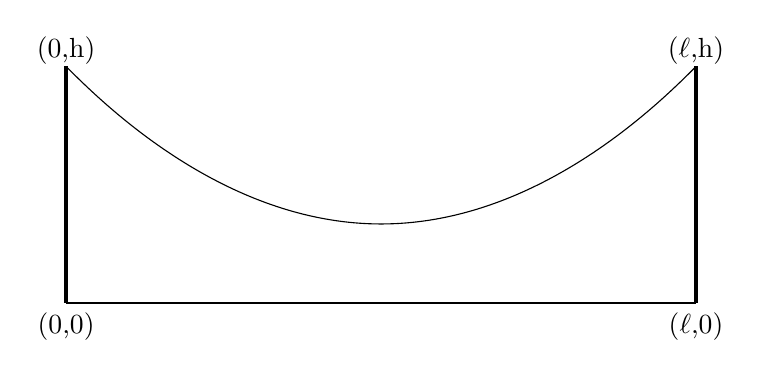
\begin{tikzpicture}
\draw[line width = 0.25mm] (1,0) -- (9,0);

\draw[line width = 0.5mm] (1,3) -- (1,0);

\draw[line width = 0.5mm] (9,3) -- (9,0);

\draw (5,1) parabola (1,3);
\draw (5,1) parabola (9,3) ;

% \draw[line width = 0.1mm] (5,0) -- (5,1);
% 
% % \draw[line width = 0.1mm] (5.5,0) -- (5.5,1.03);
% % \draw[line width = 0.1mm] (6,0) -- (6,1.1);
% % \draw[line width = 0.1mm] (6.5,0) -- (6.5,1.29);
% % \draw[line width = 0.1mm] (7,0) -- (7,1.5);
% % \draw[line width = 0.1mm] (7.5,0) -- (7.5,1.8);
% % \draw[line width = 0.1mm] (8,0) -- (8,2.1);
% % \draw[line width = 0.1mm] (8.5,0) -- (8.5,2.55);
% % 
% % \draw[line width = 0.1mm] (4.5,0) -- (4.5,1.03);
% % \draw[line width = 0.1mm] (4,0) -- (4,1.1);
% % \draw[line width = 0.1mm] (3.5,0) -- (3.5,1.29);
% % \draw[line width = 0.1mm] (3,0) -- (3,1.5);
% % \draw[line width = 0.1mm] (2.5,0) -- (2.5,1.8);
% % \draw[line width = 0.1mm] (2,0) -- (2,2.1);
% % % \draw[line width = 0.1mm] (1.5,0) -- (1.5,2.55);

\node at (1,-0.3) {(0,0)};
\node at (9,-0.3) {($\ell$,0)};
\node at (1,3.2) {(0,h)};
\node at (9,3.2) {($\ell$,h)};
\end{tikzpicture}
\caption{Side view of the main span.}
\end{figure} 

Consider the beam and elastic string in their equilibrium state. Set $w(0,t)$ as the reference points for the system. The beam has length $\ell$, and the length of the string can be calculated . 


\subsection{System of Equations}
\subsubsection{Equations of Motion}
For $x \in (0,\ell)$ and $t \in [0,T]$,
\begin{eqnarray}
\delta \partial^2_{t} u(x,t) - \partial_x V_s - k(w(x,t) - u(x,t))+ k_1 \partial_t u(x,t) = 0, \\
\rho A \partial^2_{t}w(x,t) - AG\kappa^2 \partial_xV(x,t) + k(w(x,t)-u(x,t)) + k_2\partial_t w(x,t) = 0,\\
\rho I \partial^2_{t}\phi(x,t) - EI \partial_{x} M(x,t) + AG\kappa^2V(x,t) = 0. 
\end{eqnarray}

\subsubsection{Constitutive Equations}
\begin{eqnarray}
        M &=& EI\partial_x \phi,\label{TGT_3}\\
        V &=& AG\kappa^2(\partial_x w - \phi)\label{TGT_4},\\
        V_s & = & Y\partial_x u
\end{eqnarray}

In this system, $\ell$ is the length of the beam. $w$ represents the transverse displacement of the beam's cross-section and the rotation of the cross-sections is given by $\phi$. $u$ is the vertical displacement of the elastic springs. $Y$ is the tension of the string and $\delta$ the mass per unit length. $E$ is Young's modulus, $I$ the area moment of inertia, $G$ the shear modulus, $A$ the cross-section of the beam and $\rho$ the density of the beam. $\kappa$ is the shear correction factor used with Timoshenko beam theory. $k$ represents the stiffness of the elastic spring connecting the elastic string and the beam. The terms with $k_1$ and $k_2$ represent damping terms.\\

\subsubsection{Dimensionless Equations}
The dimensionless form of the Timoshenko beam model is given is Section 1.3.4. The following dimensionless constants are introduced to add to Section 1.3.4 and allow equations (7.1) to (7.3) to be written in a dimensionless form.
\[P^* = ***, \,\, Y^* = ***, \,\, k^* = ***, \,\, k_1^* = *** \ \text{ and } \ k_2^* = ***.\]

Then the system of equations in dimensionless form is given using the original notation for convenience. 
\begin{eqnarray}
P \partial^2_{t} u(x,t) - Y\partial^2_x u(x,t) - k(w(x,t) - u(x,t))+ k_1 \partial_t u(x,t) = 0, \\
\partial^2_{t}w(x,t) - \partial^2_x w(x,t) + \partial_x\phi(x,t) + k(w(x,t)-u(x,t)) + k_2\partial_t w(x,t) = 0,\\
\frac{1}{\alpha} \partial^2_{t}\phi(x,t) - \frac{1}{\beta} \partial^2_{x} \phi(x,t) + \partial_x w(x,t) + \phi(x,t) = 0. 
\end{eqnarray}

\subsection{Boundary Conditions}
The beam is clamped elastically at the endpoints and the string is fixed at the endpoints.
\[u(0,t) = 0 \ \text{ and } \ u(1,t) = 0.\]
\[w(0,t) = 0 \ \text{ and } \ w(1,t) = 0.\]
\[\partial_x \phi(0,t) = \beta \mu\phi(0,t) \ \text{ and } \ \partial_x \phi(1,t)= \beta\mu\phi(1,t).\]

\section{Analysis of a Thermoelastic Timoshenko Beam Model}
In the article [Boc20], the authors attempt to model a single span of a suspension bridge. The bridge is modelled as a cable suspended Timoshenko beam system. The assumption for using a beam is that the length $\ell$ of the beam is large compared to the sectional dimensions so that they are negligible. In this system a beam is simply supported at the endpoints. A horizontal elastic string, representing  the main cable, is fixed at both endpoints above the beam and has the same length as the beam. A distributed force, simulating the connecting vertical cables, acts between the beam and the elastic string. This distributed force is modelled as an elastic spring, acting on the entire interval $(0,\ell)$. The beam also has thermal properties, allowing the beam to expand and contract due to temperature.\\

The system for the thermoelastic beam model is given, with updated notation. For $x \in (0,\ell)$ and $t \in [0,T]$,
\begin{eqnarray}
P \partial^2_{t} u(x,t) - Y\partial^2_x u(x,t) - k(w(x,t) - u(x,t))+ k_1 \partial_t u(x,t) = 0, \\
\textcolor{red}{\rho A \partial^2_{t}w(x,t) - AG\kappa^2 \partial_x[\partial_x w(x,t) + \phi(x,t)]} + k(w(x,t)-u(x,t)) + k_2\partial_t w(x,t) = 0,\\
\textcolor{red}{\rho I \partial^2_{t}\phi(x,t) - EI \partial^2_{x} \phi(x,t) + AG\kappa^2[\partial_x w(x,t) + \phi(x,t)]} - \mu\partial_x T(x,t) = 0,\\
\partial_t T(x,t) - \tau\partial_x^2T(x,t) - \mu \partial_{x}\partial_t\phi(x,t) = 0.
\end{eqnarray}
With boundary conditions:
\begin{eqnarray*}
 u(0,t) = w(0,t) = \phi(0,t) = T(0,t) = u(\ell,t) = w(\ell,t) = \partial_x \phi(\ell,t) = T(\ell,t) = 0
\end{eqnarray*}

In this system, $\ell$ is the length of the beam and the elastic string. $w$ represents the transverse displacement of the beam's cross-section and the rotation of the cross-sections is given by $\phi$. $u$ is the vertical displacement of the elastic string. $Y$ is the elastic modulus of the string and $P$ the mass material. $E$ is Young's modulus, $I$ the area moment of inertia, $G$ the shear modulus, $A$ the cross-section of the beam and $\rho$ the density of the beam. $\kappa$ is the shear correction factor used with Timoshenko beam theory. $k$ represents the stiffness of the elastic spring connecting the elastic string and the beam. $\mu$ is a coupling coefficient depending on the material properties. The terms with $k_1$ and $k_2$ represent damping terms, and $T$ is the thermal moment with $\tau$ the thermal diffusivity.\\

\begin{itemize}
 \item \textcolor{red}{Boundary conditions het 'n probleem}
 \item \textcolor{red}{Verduidelik nie hoekom die string horisontaal is en nie parabolies nie}
 \item \textcolor{red}{Parameters vir die elastic string moet uitgefigure word}
 \item \textcolor{red}{Dimensieloosheid}
\end{itemize}


************************Nog Net in gecopy**********************
\subsubsection{Dimensionless Equations}

Set \[\tau = \frac{t}{t_0}, \,\, \xi = \frac{x}{\ell}, \,\, u^*(\xi,\tau) = \frac{u(x,t)}{\ell} \ \text{ and } \ \phi^*(\xi, \tau) = \phi(x,t).\]

The dimensionless forms of the shear force, moment and load are \[ V^{*}(\xi,\tau) = \frac{V(x,t)}{AG\kappa^2}, \quad M^{*}(\xi,\tau) = \frac{M(x,t)}{A G\kappa^2 \ell} \,\,\, \ \text{and} \ \,\,\, Q^*(\xi,\tau) = \frac{Q(x,t)\ell}{A G\kappa^2}.\]

Choose $t_0$ the same as in Section 1.3.4, i.e. \[t_0 = \ell\sqrt{\frac{\rho}{G\kappa^2}}.\]

We introduce the dimensionless constants
\begin{equation*}
\alpha = \frac{A \ell^2}{I} \,\,\, \text{and} \,\,\, \beta
=\frac{AG\kappa^2 \ell^2}{EI}.
\end{equation*}

We also have the relation $\gamma = \frac{\beta}{\alpha}$.\\
********************************************************\\

\section{An Elastically Clamped Beam Model}
Consider the following equations of motion and constitutive equations for a Cantilever Timoshenko Beam that is clamped elastically at both endpoints.
\subsubsection*{Equations of Motion}
\begin{eqnarray}
	\partial_t^2 w &=& \partial_x V - c_1\partial_t w  +q, \label{CT_1}\\
	\frac{1}{\alpha}\partial_t^2 \phi &=& V+\partial_xM. \label{CT_2}
\end{eqnarray}

\noindent
\subsubsection*{Constitutive Equations}
\begin{eqnarray}
	M &=& \frac{1}{\beta}\partial_x \phi +c_2 \partial_t \partial_x \phi,\label{CT_3}\\
	V&=& \partial_x w - \phi.\label{CT_4}
\end{eqnarray}
The terms with $c_1$ represents vicous damping, and the term with $c_2$ represents material damping.\\

\subsubsection{Boundary Conditions}
\noindent
The boundary conditions at the (elastically) clamped ends are
\begin{eqnarray}
   w(x,\cdot) &=&  0, \label{CT_5}\\
   M(x,\cdot) &=&  \mu \phi(x,\cdot). \label{CT_6}
\end{eqnarray} at $x = 0$ and $x = 1$.\\

With these boundary conditions, $\mu$ models the elastic interaction between the surface where the beam is attached and the beam itself. As $\mu$ increases, $\phi(0,t)$ decreases and similarly as $\mu$ decreases, $\phi(0,t)$ increases. This implies the the cross-section at $x=0$ will rotate less with a larger $\mu$ hence the elastic join is `more' rigid, and the cross-section will rotate more with a smaller $\mu$, hence a `more' elastic join.\\

Consider the general form of plane stress from Section \ref{ssec:3D_Model:PlaneStress}. As mentioned in \cite{Fung65}, this is not a true two-dimensional model. Using the definition of strain \eqref{eq:3D_Model:Strain} and assuming plane stress parallel to the $e_1$-$e_2$ plane,
\begin{eqnarray}
	\varepsilon_{13} &=&  \frac{1}{2}\left( \frac{\partial u_1}{\partial x_3} + \frac{\partial u_3}{\partial x_1} \right) = 0,\label{e_1}\\
	\varepsilon_{23} &=& \frac{1}{2}\left( \frac{\partial u_2}{\partial x_3} + \frac{\partial u_3}{\partial x_2} \right) = 0,\label{e_2}\\
	\varepsilon_{33} &=& \frac{\partial u_3}{\partial x_3}.\label{e_3}
\end{eqnarray}
Hence $u_1$ and $u_2$ are functions of $x_1$, $x_2$ and $x_3$, and $u_3$ is linear function with respect to $x_3$. Therefore the model is still three-dimensional in the case of general plane stress. More assumptions are required to obtain a true two-dimensional model.\\

Assume that $\sigma_{3i} = 0$ for $i = 1,2,3$ (minimum assumption for plane stress). Also assume $u_1$ and $u_2$ are functions of $x_1$ and $x_2$ only, and that the strain component $\epsilon_{33} = 0$. From \eqref{e_1} - \eqref{e_3}, it follows that
\begin{eqnarray*}
	\frac{\partial u_3}{\partial x_i} & = & 0  \ \ \ \ \textrm{ for } i = 1,2,3 \textrm{ on } \Omega.
\end{eqnarray*} 
Therefore $u_3$ is a constant and the model is two-dimensional.

\subsubsection{Hooke's law in two-dimensions}
Using the components components \eqref{stress_comp} of the stress tensor $T$, Hooke's Law \eqref{eq:3D_Model:CE-D} in two-dimensions can be written as 
\begin{eqnarray}
	T = \frac{1}{\gamma(1+\nu)}\mathcal{E} + \frac{\nu}{\gamma(1-\nu^2)}\textrm{tr}(\mathcal{E}) I. 
\end{eqnarray}


\end{document}
